\documentclass[conference]{IEEEtran}

\IEEEoverridecommandlockouts %To add sponsors and index terms

\usepackage{cite}

\ifCLASSINFOpdf
   \usepackage[pdftex]{graphicx}
  % declare the path(s) where your graphic files are
%   \graphicspath{{../images/}}
  % and their extensions so you won't have to specify these with
  % every instance of \includegraphics
   \DeclareGraphicsExtensions{.pdf,.jpeg,.png}
\else
\fi

\usepackage[cmex10]{amsmath}
%\usepackage[hidelinks]{hyperref}
\usepackage{nohyperref}
\usepackage{url}
%for columns spanning multiple rows in tables
\usepackage{multirow}
%use the booktabs package to get (much!) better vertical spacing above and below "rules" (horizontal lines), resulting in a much more professional look of your tables.
%use the colortbl package to add color to tables.
\usepackage{booktabs,colortbl}

\usepackage{amsfonts}

% correct bad hyphenation here
\hyphenation{op-tical net-works semi-conduc-tor}

  \renewcommand\footnoterule{\vspace*{-3pt}%
     \hrule width 2in height 0.4pt
     \vspace*{2.6pt}}

\begin{document}
%
% paper title
% can use linebreaks \\ within to get better formatting as desired
\title{The Journal Article:\\
subtitle}


% author names and affiliations
% use a multiple column layout for up to two different
% affiliations
\author{%

\IEEEauthorblockN{Jonas Kersulis,\\ Ian Hiskens}
%\IEEEauthorblockA{Electrical Engineering and Computer Science\\
\IEEEauthorblockA{Elec. Eng. and Computer Science \\
University of Michigan\\
Ann Arbor, MI, United States\\}
\and
\IEEEauthorblockN{Michael Chertkov,\\Scott Backhaus}
%\IEEEauthorblockA{Center for Nonlinear Studies\\
\IEEEauthorblockA{Center for Nonlinear Studies\\
Los Alamos National Laboratory\\
Los Alamos, NM, United States\\
}
\and
\IEEEauthorblockN{Daniel Bienstock\\ \hspace{1pt} }
%\IEEEauthorblockA{Industrial Engineering and Operations Research\\
\IEEEauthorblockA{Ind. Eng. and Operations Research\\
Columbia University\\
New York, NY, United States\\
}

% use \thanks{} to gain access to the first footnote area
% a separate \thanks must be used for each paragraph as LaTeX2e's \thanks
% was not built to handle multiple paragraphs

% Who are our sponsors?
%\thanks{Identify applicable sponsor/s here. \emph{(sponsors)}}%
\thanks{The authors acknowledge the support of the Los Alamos National Laboratory Grid Science Program, subcontract 270958.}%
}

% make the title area
\maketitle

%ABSTRACT
\begin{abstract}
%A time-coupled instanton method for characterizing transmission network vulnerability to wind generation fluctuation is presented. To extend prior instanton work to multiple-time-step analysis, line constraints are specified in terms of temperature rather than current. An optimization formulation is developed to express the minimum wind forecast deviation such that at least one line is driven to its thermal limit. Results are shown for an IEEE RTS-96 system with several wind-farms.
A previously-developed method for studying a transmission network's vulnerability to wind forecast inaccuracy is expanded. This method uses optimization to find a wind generation pattern close to the forecast that violates a specified line. Repeating the optimization for all lines in the network yields a set of generation patterns which may be sorted by likelihood. Instanton analysis thus yields insight into the potential effects of wind forecast inaccuracy at the system level.
\end{abstract}

%INDEX TERMS
% The author shall provide up to 4 keywords (in alphabetical order) to help identify the major topics of the paper. The thesaurus of IEEE indexing keywords is posted at http://www.ieee.org/organizations/pubs/ani_prod/keywrd98.txt
\begin{IEEEkeywords}
Forecast uncertainty, Optimization, Transmission operations, Wind energy
\end{IEEEkeywords}


\section{Introduction and review}\label{sec:intro}

The impact of wind forecast inaccuracy is greater than ever in grids around the world. As reliance on wind generation increases, changes in weather can induce network congestion. In certain cases this congestion may even cause a transmission line to overheat and sag. System operators use wind forecast data to steer the network away from these scenarios, but wind forecasts are significantly less accurate than generation and demand predictions. How might forecast inaccuracies compound across the network to overheat transmission lines? How likely is this to occur? In this paper we develop temporal instanton analysis, which uses mathematical programming to find troublesome wind patterns and rank them according to likelihood. With this information, system operators and planners gain a new line of defense against renewable generation uncertainty.

The remainder of this paper is organized as follows. Section II translates the verbal description above into a mathematical formulation of temporal instanton analysis. Section III describes a previously-developed solution method for the temporal instanton problem. We expand on prior work by providing a more detailed treatment of the objective function, discussing implementation details including computational complexity and sparsity, and proposing a particular algorithm for solving the secular equation. Section IV contains results for two networks: a modified version of the RTS-96 and the larger WECC network. The former network has been used in previous instanton analysis studies, while the latter serves to demonstrate scalability of temporal instanton analysis. Finally, an appendix contains a detailed description of the thermal model used to calculate line temperature.

Wind forecasting is a complicated business. Consider first a single wind farm whose output is forecast for some future time. Let the forecast performance be represented by a random variable. Using historical data from ERCOT in Texas, \cite{hodge2011} determined appropriate density functions for this variable based on the forecast horizon. For predictions a few minutes or hours away, forecast performance is approximately Cauchy, with deviations concentrated heavily around the forecast value. As the time horizon increases, accuracy suffers and the distribution approaches the Gaussian curve. Now consider several wind farms scattered across a transmission grid. In addition to individual site forecasts, one must now consider overall patterns. Wind sites tend to be spatially correlated: if wind speed increases at one site, it is unlikely that it will simultaneously decrease at a neighboring site. Temporal correlation further complicates matters: increased wind at site A now may be strongly correlated with greater wind speeds at site B in the future. Spatial and temporal correlation may be calculated from measurement data and encoded in a correlation matrix. The optimization framework developed in this paper contains such a correlation matrix in its objective function.

%The prevalence of renewables in modern transmission networks has
%researchers and system operators asking: What happens when the wind
%changes, and could fluctuations harm the grid? The instanton problem
%provides an answer, and this paper extends instanton analysis to the
%temporal setting. Though small deviations from wind forecasts are
%typically harmless, it is possible for certain wind generation
%patterns to drive the system to an insecure operating point. Out of
%all troublesome wind generation patterns, the one that deviates least
%from the forecast is called the instanton. Instanton analysis uses
%optimization to find the set of troublesome wind patterns, each of
%which causes a particular line to encounter its flow limit. By
%ranking these wind patterns according to distance from forecast, we
%can characterize the system's vulnerability to forecast inaccuracy and
%enhance system operator awareness.
%
%The instanton problem was initially considered in \cite{chertkov2011}
%and \cite{chertkov2011a} where a DC power flow approximation was used
%to turn instanton analysis into a convex problem with an analytic
%solution. The physically accurate AC power flow formulation was used
%in \cite{baghsorkhi2012}, with an iterative scheme required for
%finding instanton candidates. Current instanton research is exploring
%the trade-off between problem complexity and solution accuracy, with
%the goal of developing the most accurate model that remains convex
%(and therefore guarantees a solution).  Instanton work to date has
%focused on instantaneous vulnerability by seeking to find the smallest
%wind generation change that drives a line to its power or current
%limit. Thus, the troublesome wind patterns uncovered by such instanton
%analysis may be fleeting.
%
%It is safe to temporarily operate a line above its current
%limit. Transmission system operators know this and periodically allow
%lines to operate above their limits to promote smooth operation under
%heavy, though temporary, flow patterns (see the introduction of
%\cite{banakar2005} for a history of dynamic line rating starting in
%the 1970s). It takes time for line conductors to heat sufficiently
%that they sag to an unacceptable level (as defined by statute and
%nearby tree limbs). As long as the line is allowed to cool before
%reaching this point, no harm will be done. If an operator is
%comfortable with temporarily overloaded lines, information from
%existing instanton analysis may be too conservative to aid decision
%making.
%
%In this paper we bring instanton analysis into the temporal
%setting. We consider multiple time steps and replace line current
%limits with heat constraints. A line's temperature is a function of
%heat input (primarily Ohmic losses and heat from the sun) and
%dissipation (convection and radiation, which depend on ambient
%conditions), and is represented as a differential equation (see
%Section 3.4 of \cite{ieee2007} for a standard set of equations
%governing line temperature dynamics). Ohmic loss heating is related to
%power flow analysis via angle difference variables. By modeling line
%temperature over an appropriate time horizon, the proposed method
%discovers multiple-time-step wind patterns that are both likely to
%occur and sure to induce excessive sag for at least one line in the
%network.

%The remainder of the paper describes the temporal instanton problem (Section \ref{sec:problem}), translates it into an optimization problem (Section \ref{sec:optimization}), presents a solution method (Section \ref{sec:solution}), and illustrates temporal instanton analysis using a modified RTS-96 network (Section \ref{sec:results}).
%Instanton analysis may also be viewed as an optimal control problem. The goal is to drive the system to the edge of its feasible operating region while minimizing the ``effort'' of wind variation. We want to find the smallest deviation from a wind forecast that will drive enough current through at least one line to send it to its thermal limit. It is easy to check whether a particular wind forecast will lead to a line exceeding its thermal threshold; instanton analysis provides us with the sensitivity of line overloads to changes in the given forecast.
%If the relationship between generation and heat input was linear, we would have a linear optimal control problem.

\section{Temporal instanton problem as a QCQP}\label{sec:qcqp}

\subsection{Line losses}\label{sec:line-losses}

Starting with the AC line loss expression, \cite{almassalkhi2014}
derived the following approximate relationship between line losses and
voltage angle differences for line $(i,j)$:
\begin{equation}
\label{LL:activeLoss}
f_{ij}^{\text{loss}} \approx r_{ij}\left(\frac{\theta_{ij}}{x_{ij}}\right)^2.
\end{equation}
In this expression, $f_{ij}^{\text{loss}}$ is the approximate active
power loss on the line; $\theta_{ij}$ is the difference between angles
$\theta_i$ and $\theta_k$; and $r_{ij} +j x_{ij}$ is the impedance of
the line between nodes $i$ and $j$. Three assumptions underpin
\eqref{LL:activeLoss}: voltage magnitudes are all 1~pu, cosine may be
approximated by its second-order Taylor expansion, and $x_{ij} \geq
4r_{ij}$. Thus, \eqref{LL:activeLoss} uses DC power flow assumptions
to approximate line losses, but remains nonlinear.

\subsection{Objective function and $Q_{obj}$}\label{sec:Qobj}

The objective function depends solely on deviation variables, so
$Q_{obj}$ is a matrix that weights only the $dev$ variables in $z$. If
there are two time steps, for example, the vector of variables would
be $z = \begin{bmatrix}dev_t^\top & \theta_1^\top & \alpha_1 &
  dev_2^\top & \theta_2^\top & \alpha_2 &
  \hat{\theta}\end{bmatrix}^\top$, and $Q_{obj}$ would be,
\begin{align*}
Q_{obj} = \begin{bmatrix} Q_{dev} & 0 & 0 & 0 & 0 & 0 \\ 0 & 0 & 0 & 0 & 0 & 0 \\ 0 & 0  & 0 & 0 & 0 & 0 \\ 0 & 0 & 0 & Q_{dev} & 0 & 0 \\ 0 & 0 & 0 & 0 & 0 & 0 \\ 0 & 0 & 0 & 0 & 0 & 0\end{bmatrix}.
\end{align*}
Note that $Q_{dev}$ represents the correlation between wind-farms (if any). In the Section \ref{sec:solution} numerical analysis, we will assume $Q_{dev}=I$, the identity matrix.

\subsection{Linear constraints: $A$ and $b$}\label{sec:Ax=b}

All constraints except the temperature limit may be grouped into a single linear system $Az=b$. Setting aside the $T$ auxiliary variables for the moment, the $A$ matrix has a block diagonal structure where each block consists of $(N+1)$ rows and $(N_R+N)$ columns. The first $N$ rows describe power balance and distributed slack behavior at each node. For node $i$ and time $t$, we fix elements of $A$ and $b$ to establish
\begin{equation}\label{pbal}
\sum\limits_{j} Y_{ij}\theta_{j,t}  = (G_{i,t}^0 + k_i\alpha_t) +
(R_{i,t} + dev_{i,t}) - D_{i,t}.
\end{equation}
The first pair of terms on the right-hand side of \eqref{pbal}
represents conventional generation with distributed slack (generator
$i$ is taking a portion $k_i$ of the mismatch $\alpha_t$). The second
pair of terms is renewable generation: forecast $R_{i,t}$ plus
deviation $dev_{i,t}$. The final term is demand at node $i$ and time
$t$. (Note that renewable generation terms are zero for nodes without
wind-farms.) In addition to the $N$ rows corresponding to \eqref{pbal}
at the $N$ nodes, there is one additional equation associated with
time $t$ that fixes the angle reference:
\begin{equation}\label{mismatch}
\theta_{ref,t} = 0.
\end{equation}

The $(N+1)$ rows of $Az=b$ expressed in \eqref{pbal} and
\eqref{mismatch} pertain to a single time step $t$, with $T$ blocks of
this form arranged diagonally to form $(N+1)T$ rows of $A$ and the
corresponding $b$ vector. There is one additional block of $A$ used to
define auxiliary angle difference variables $\hat{\theta}_{ij,t}$ in
terms of angle variables $\theta_{i,t}$ and $\theta_{j,t}$ at each
time step:
\begin{align}\label{thetahat}
\hat{\theta}_{ij,t} &= \tau^{\frac{T-t}{2}}(\theta_{i,t} - \theta_{j,t})~.
\end{align}
The next subsection explains why these variables are helpful.

\subsection{Quadratic constraint: $Q_{\theta}$ and $c$}\label{sec:Qtheta}

Recall that \eqref{temp} describes the temperature constraint on a
chosen line $(i,j)$. We can rearrange \eqref{temp} into the form of
\eqref{opt:quad}, with all constants on the right side:
\begin{equation}\label{temp2}
\boldsymbol{\theta}_{ij}^\top \boldsymbol{\tau}_{ij} \boldsymbol{\theta}_{ij} =  \frac{x_{ij}^2}{\rho_{ij} r_{ij}} \left(\Delta T_{ij}^{\text{lim}} - \delta_{ij} \boldsymbol{\Delta d}_{ij}^\top \boldsymbol{\tau}_{ij}\mathbf{1}\right)
\end{equation}
This makes it clear that the appropriate value of $c$ in \eqref{opt:quad} is
\begin{equation}
c = \frac{x_{ij}^2}{\rho_{ij} r_{ij}} \left(\Delta T_{ij}^{\text{lim}} - \delta_{ij} \boldsymbol{\Delta d}_{ij}^\top \boldsymbol{\tau}_{ij}\mathbf{1}\right)
\end{equation}
From the definition of $\hat{\theta}_{ij,t}$ in \eqref{thetahat}, we see that the left side of \eqref{temp2} may be expressed as $\hat{\theta}_{ij}^\top \hat{\theta}_{ij}$. Thus, if the $\hat{\theta}_{ij}$ variables are placed at the bottom of $z$, $Q_{\theta}$ must be a matrix of zeros with a $T$-by-$T$ identity matrix in the lower-right corner. This ensures that $z^\top Q_\theta z = \hat{\theta}_{ij}^\top\hat{\theta}_{ij}$, as desired.

Section \ref{sec:problem} described the temporal instanton problem, Section \ref{sec:optimization} expressed it as a QCQP, and this section defined each component. Next we present a solution method for \eqref{opt}.


\section{Solution method and implementation details}\label{sec:solution}

The structure of \eqref{opt} is similar to that of the well-known trust region subproblem. Here we describe a four-step solution method based in part on \cite{bienstock2014}. We begin by considering the vector of variables $z$ as three groups: $z_1\in\mathbb{R}^{N_RT}$ contains all wind deviations, $z_2\in\mathbb{R}^{(N+1)T}$ contains angle and mismatch variables, and $z_3\in\mathbb{R}^T$ contains auxiliary angle difference variables involved in line temperature calculation. (This partition of $z$ is independent of how the variables are ordered.) With this notation, the problem becomes
\begin{subequations}\label{optpart}
\begin{align}
\min\quad z_1^\top &Q_z z_1 \\
s.t.\quad Az &= b \\
z_3^\top z_3 &= c,
\end{align}
\end{subequations}
where $Q_z$ is $Q_{dev}$ repeated in block-diagonal fashion $T$ times.

Several changes of variables may be used to obtain an equivalent form
of \eqref{optpart} whose solution is straightforward.

\subsection{Translation}

The first step is to change variables from $z$ to $y=z-z^*$, where
$z^*\in\{z:Az=b\}$. This translation transforms $Az=b$ into $Ay=0$. To
prevent the change from introducing a linear term into the quadratic
constraint, we require $z_3^*=0$. To satisfy $Az^*=b$, the subvectors
$z_1^*$ and $z_2^*$ must satisfy,
\[
A \begin{bmatrix} z_1^* \\ z_2^*
\\ 0 \end{bmatrix} = b.
\]
It is straightforward to find a min-norm $z^*$ that satisfies this
constraint by partitioning and factorizing $A$ appropriately. After
translation, the problem becomes
\begin{subequations}\label{opt2}
\begin{align}
\label{opt2:obj} \min\quad y_1^\top &Q_z y_1 + 2 y_1^\top Q_z z_1^* \\
\label{opt2:lin} s.t.\quad Ay &= 0 \\
\label{opt2:quad} y_3^\top y_3 &= c.
\end{align}
\end{subequations}

\subsection{Kernel mapping}

The form of \eqref{opt2:lin} suggests an intuitive explanation: any
solution to \eqref{opt2} must lie in the nullspace (kernel) of $A$. If
$\dim \mathcal{N}(A) =k$ is the dimension of this nullspace, we can
let $y=Nx$ where the $k$ columns of $N$ span $\mathcal{N}(A)$. (Note
that $x$ does not refer to reactance in this context.) This change of
variables is akin to a rotation, but reduces the problem dimension to
$k$. Partitioning $N$ according to,
\[
\begin{bmatrix} y_1 \\ y_2 \\ y_3 \end{bmatrix} = \begin{bmatrix} N_1
  \\ N_2 \\ N_3 \end{bmatrix} x
\]
allows \eqref{opt2} to be written,
\begin{subequations}\label{opt3}
\begin{align}
\label{opt3:obj} \min\quad  &x^\top (N_1^\top Q_zN_1) x + 2x^\top
(N_1^\top Q_zz_1^*) \\
\label{opt3:quad} s.t.\quad &x^\top N_3^\top N_3 x = c.
\end{align}
\end{subequations}
All feasible solutions to \eqref{opt3} lie in the nullspace of $A$, so
the linear constraints are now implicit.

\subsection{Obtaining a norm constraint}

After kernel mapping, the quadratic constraint is no longer a norm
constraint. This can be corrected in two steps. First, perform an
eigendecomposition $N_3^\top N_3 = UDU^\top$ and let $\hat{x} = U^\top
x$. The constraint is diagonal in terms of $\hat{x}$:
\begin{equation}
\label{opt3:rotquad} x^\top N_3^\top N_3 x = \hat{x}^\top D\hat{x}
\end{equation}
where $D$ is diagonal and has at most $T$ nonzero elements, so the
right side of \eqref{opt3:rotquad} may be expanded into:
\begin{equation}
\begin{bmatrix}
\hat{x}_1^\top & \hat{x}_2^\top \end{bmatrix}
\begin{bmatrix} 0 & 0 \\ 0 & \hat{D} \end{bmatrix}
\begin{bmatrix}
\hat{x}_1 \\ \hat{x}_2
\end{bmatrix}.
\end{equation}
The second step is to change variables from $\hat{x}$ to $w =
[w_1^\top \; w_2^\top]^\top$. The variables $x$, $\hat{x}$ and $w$ are
related through:
\begin{align}
\label{eq:x_to_w} \begin{bmatrix} w_1 \\ w_2 \end{bmatrix} &=
\begin{bmatrix} I & 0 \\ 0 & \hat{D}^{1/2} \end{bmatrix}
\begin{bmatrix} \hat{x}_1 \\ \hat{x}_2 \end{bmatrix} = K\hat{x} \\
\nonumber \implies w &= KU^\top x.
\end{align}
(Note that $x = UK^{-1}w$ because $UU^\top = I$.) In terms of $w$,
\eqref{opt3:quad} is transformed through \eqref{opt3:rotquad} to give
the form of a norm:
\begin{equation}
\hat{x}^\top D\hat{x} = \hat{x}_2^\top \hat{D}^{1/2}\hat{D}^{1/2}\hat{x}_2
= w_2^\top w_2~.
\end{equation}
Of course, this change of variables must also be applied to the cost function. After substitution and simplification, the full problem becomes:
\begin{subequations}\label{opt4}
\begin{align}
\label{opt4:obj} \min\quad &w^\top Bw + w^\top b \\
\label{opt4:quad} s.t.\quad &w_2^\top w_2 = c
\end{align}
\end{subequations}
where 
\[
B= K^{-1}U^\top N_1^\top Q_z N_1 UK^{-1} \text{ and }b=2 K^{-1}U^\top
N_1^\top Q_z z_1^*.
\]

The manipulations in this section have restored the norm structure of
the quadratic constraint. In the next section we use the KKT
conditions of \eqref{opt4} to eliminate $w_1$, the unconstrained part
of $w$. This will allow us to write the objective in terms of $w_2$
only.

\subsection{Eliminating $w_1$}

Note that $w_1$ is unconstrained in \eqref{opt4}. For a fixed $w_2$, we can use the KKT
conditions to find $w_1$ such that the objective is minimized. Begin by
expanding the objective:
\begin{align*}
f(w) &=
\begin{bmatrix} w_1^\top & w_2^\top \end{bmatrix}
\begin{bmatrix} B_{11} & B_{12} \\ B_{12}^\top & B_{22}\end{bmatrix}
\begin{bmatrix} w_1 \\ w_2 \end{bmatrix} + 
\begin{bmatrix} w_1^\top & w_2^\top \end{bmatrix}
\begin{bmatrix} b_1 \\ b_2\end{bmatrix} \\
&=
w_1^\top B_{11}w_1 + 2w_1^\top B_{12}w_2 + w_2^\top B_{22}w_2 \\
&\qquad + w_1^\top b_1 + w_2^\top b_2.
\end{align*}
Next, set the partial derivative with respect to $w_1$ equal to zero:
\begin{align}
\nonumber \frac{\partial f}{\partial w_1} &= 2w_1^\top B_{11} + 2w_2^\top B_{12}^\top + b_1^\top = 0 \\
\label{eq:elimw1} \implies w_1 &= -B_{11}^{-1}\left(B_{12}w_2 +
\frac{1}{2}b_1 \right).
\end{align}
After substitution of \eqref{eq:elimw1}, the objective depends only on $w_2$:
\begin{align*}
f(w_2) &= w_2^\top\left(B_{22} - B_{12}^\top B_{11}^{-1}
B_{12}\right)w_2 \\
&\qquad + w_2^\top (b_2 - B_{12}^\top B_{11}^{-1}b_1).
\end{align*}
%\begin{align*}
%f(w_2) &= w_2^\top\left(B_{22} - B_{12}^\top B_{11}^{-1} B_{12}\right)w_2 + 
%w_2^\top (b_2 - B_{12}^\top B_{11}^{-1}b_1) \\
%&\qquad - \frac{1}{4}b_1^\top B_{11}^{-1}b_1
%\end{align*}
(Note that the constant term, which plays no role in minimization, was
omitted.) The full optimization problem becomes:
\begin{subequations}\label{opt5}
\begin{align}
\min\quad & w_2^\top \hat{B}w_2 + w_2^\top \hat{b} \\
\label{opt5:quad} s.t.\quad & w_2^\top w_2 = c,
\end{align}
\end{subequations}
where
\[
\hat{B} = B_{22} - B_{12}^\top B_{11}^{-1}B_{12} \text{ and }\hat{b} = b_2 - B_{12}^\top B_{11}^{-1}b_1.
\]
This is a QCQP in $T$ dimensions with a single norm constraint. It is
straightforward to obtain solutions to this problem, as the next
subsection shows.

\subsection{Solution via enumeration}

A straightforward method of solving \eqref{opt5} involves initially
diagonalizing $\hat{B}$ through an eigendecomposition. It will be
assumed that step has been completed.

Let $v$ be the Lagrange multiplier associated with \eqref{opt5:quad}
and write the first-order optimality condition for \eqref{opt5}:
\begin{align}
\nonumber \frac{\partial \mathcal{L}(w_2,v)}{\partial w_2} &= 2\hat{B}w_2 + \hat{b} - v(2w_2) = 0 \\
\label{opt5:kkt} \implies \hat{B}w_2 + \frac{1}{2}\hat{b} &= vw_2.
\end{align}
Equation \eqref{opt5:kkt} is a linear system that yields $w_2$ for fixed $v$:
\begin{equation}
\label{opt5:kkt2}w_{2,i} = \frac{\hat{b}_i/2}{v - \hat{B}_{i,i}}.
\end{equation}
In addition to satisfying \eqref{opt5:kkt2}, an optimal $w_2$ must
satisfy the quadratic constraint. Substituting \eqref{opt5:kkt2} into
\eqref{opt5:quad} yields the ``secular equation'' (see
\cite{bienstock2014}):
\begin{equation}
s(v) = \sum_{i}\left( \frac{\hat{b}_i /2}{v - \hat{B}_{i,i}}\right)^2 = c.
\end{equation}
Note that $s(v)$ has one pole per unique nonzero diagonal element of
$\hat{B}$. There are at most two solutions per pole, one on each
side. This is best understood graphically. Figure \ref{fig:secular}
illustrates a three-pole secular equation taken from analysis of the
RTS-96 network. The Lagrange multiplier $v$ is on the horizontal axis,
and the secular equation value $s(v)$ is on the vertical. Solutions
are intersections of $s(v)$ with the horizontal line $s(v)=c$. They
can be computed numerically with a simple binary search algorithm.

\subsection{Computation complexity}

\subsection{Sparsity}

\section{Results}\label{sec:results}

We used data from \cite{pandzic} to demonstrate temporal instanton
analysis on a wind-augmented RTS-96 network model. Consider a scenario
unfolding over three time steps: first the wind forecast is 50\% of
some nominal value, next it is equal to the nominal value, and finally
it is scaled to 150\% of nominal. Throughout this wind ramping,
generator dispatch and demand remain constant. Temporal instanton
analysis with $c=0.03$ and $\tau=0.5$ indicates that the line between
buses 121 and 325 is most susceptible to excessive heating under these
conditions. In other words, of all dangerous wind patterns that could
occur during the wind ramp, the most likely is a pattern that
overheats the line between buses 121 and 325. Figure~\ref{fig:secular}
illustrates the secular equation used to find this instanton pattern,
and Figure~\ref{fig:line118} shows the system state at the second time
step. The largest deviation in the instanton pattern is $0.73$ pu,
well within the range of wind forecast values (whose maximum is $1.2$
pu).


\begin{figure}[t]
\centering
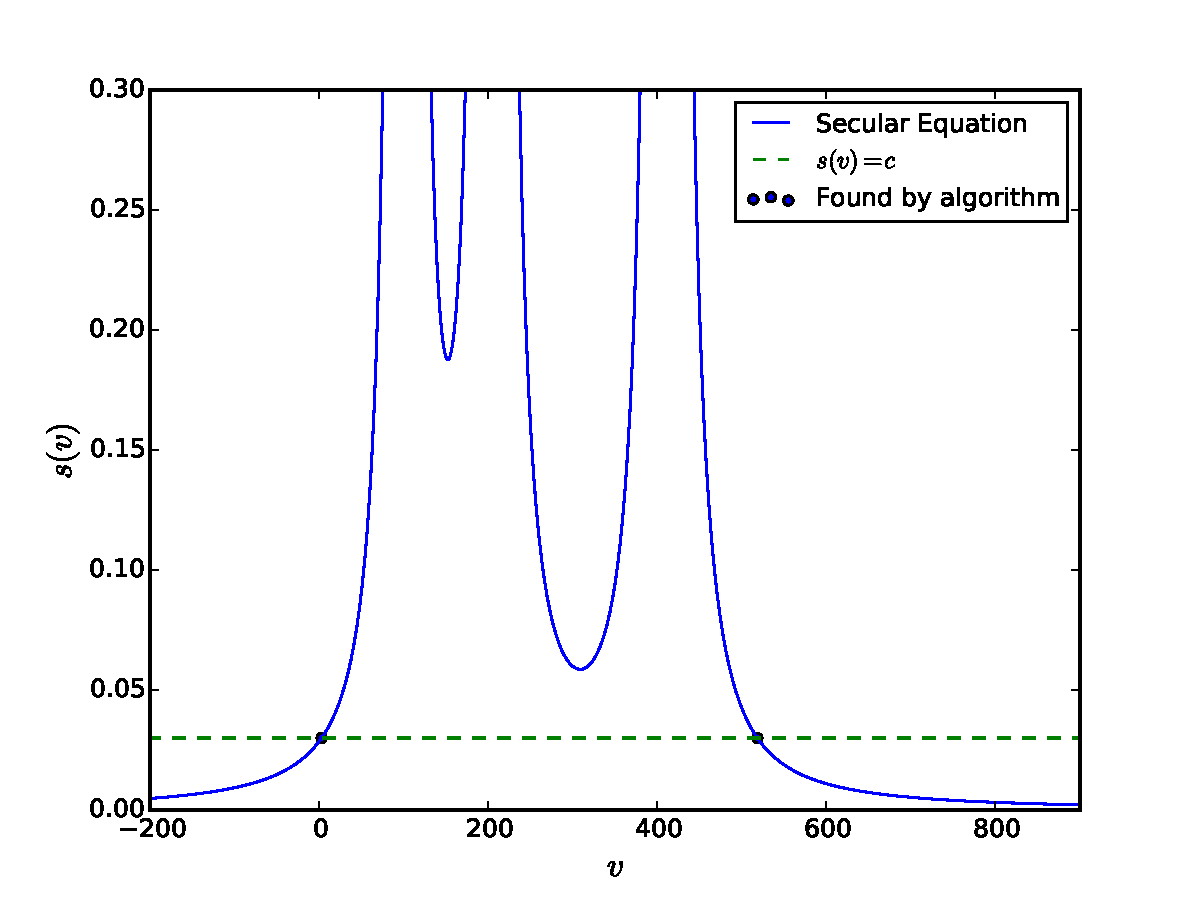
\includegraphics[trim=0in 0in 0.5in 0.5in,clip,width=1\linewidth]{images/secular}
\caption{Plot of secular equation for a single line in the RTS-96. Note that $s(v)$ approaches infinity at the three poles, and there could be as many as six solutions if $c$ were large enough.}	
\label{fig:secular}
\end{figure}

%\begin{figure}
%\centering
%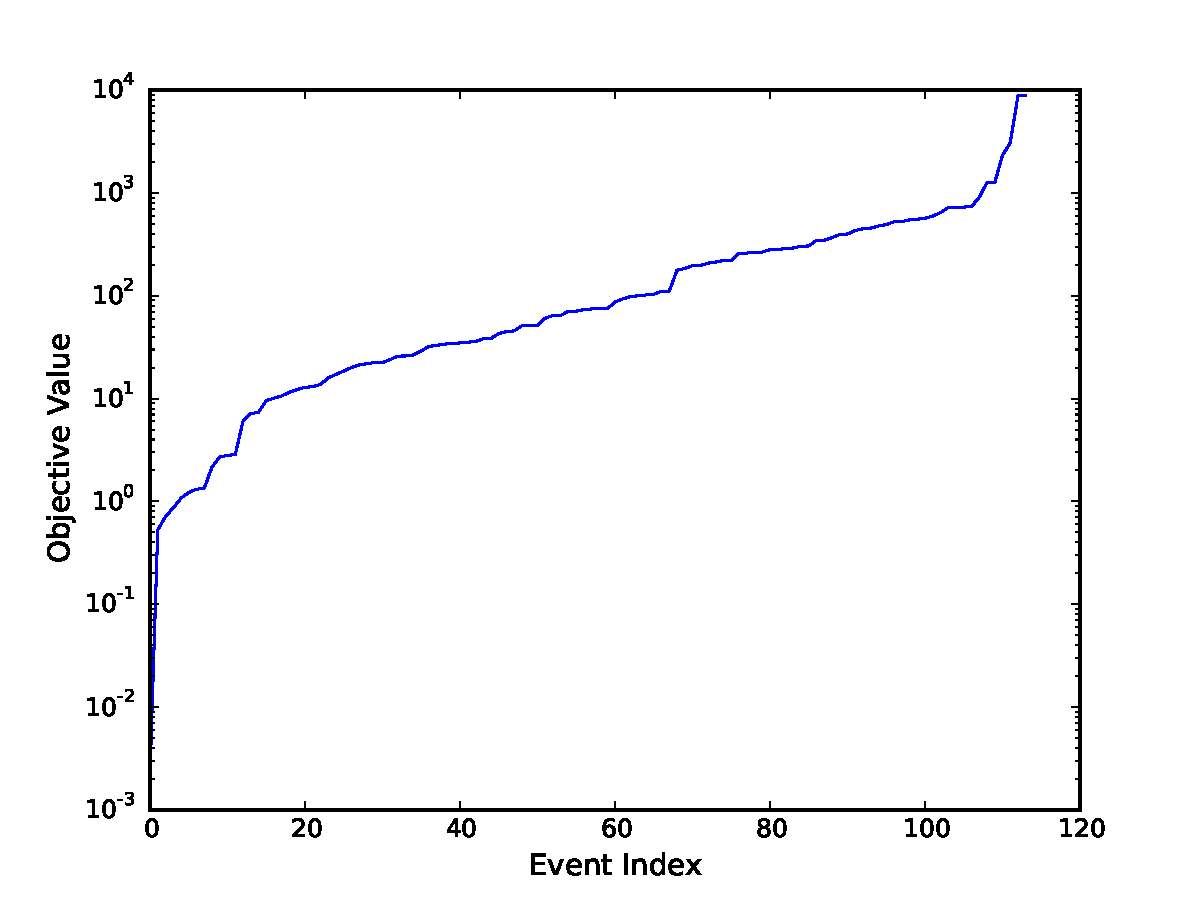
\includegraphics[width=1\linewidth]{../images/scores}
%\caption{Semilogarithmic plot of sorted objective values for RTS-96 temporal instanton analysis. (Note that six lines are missing objective values. The algorithm did not produce solutions for these lines due to numerical instability.)}
%\label{fig:scores}
%\end{figure}

\begin{figure}[t]
\centering
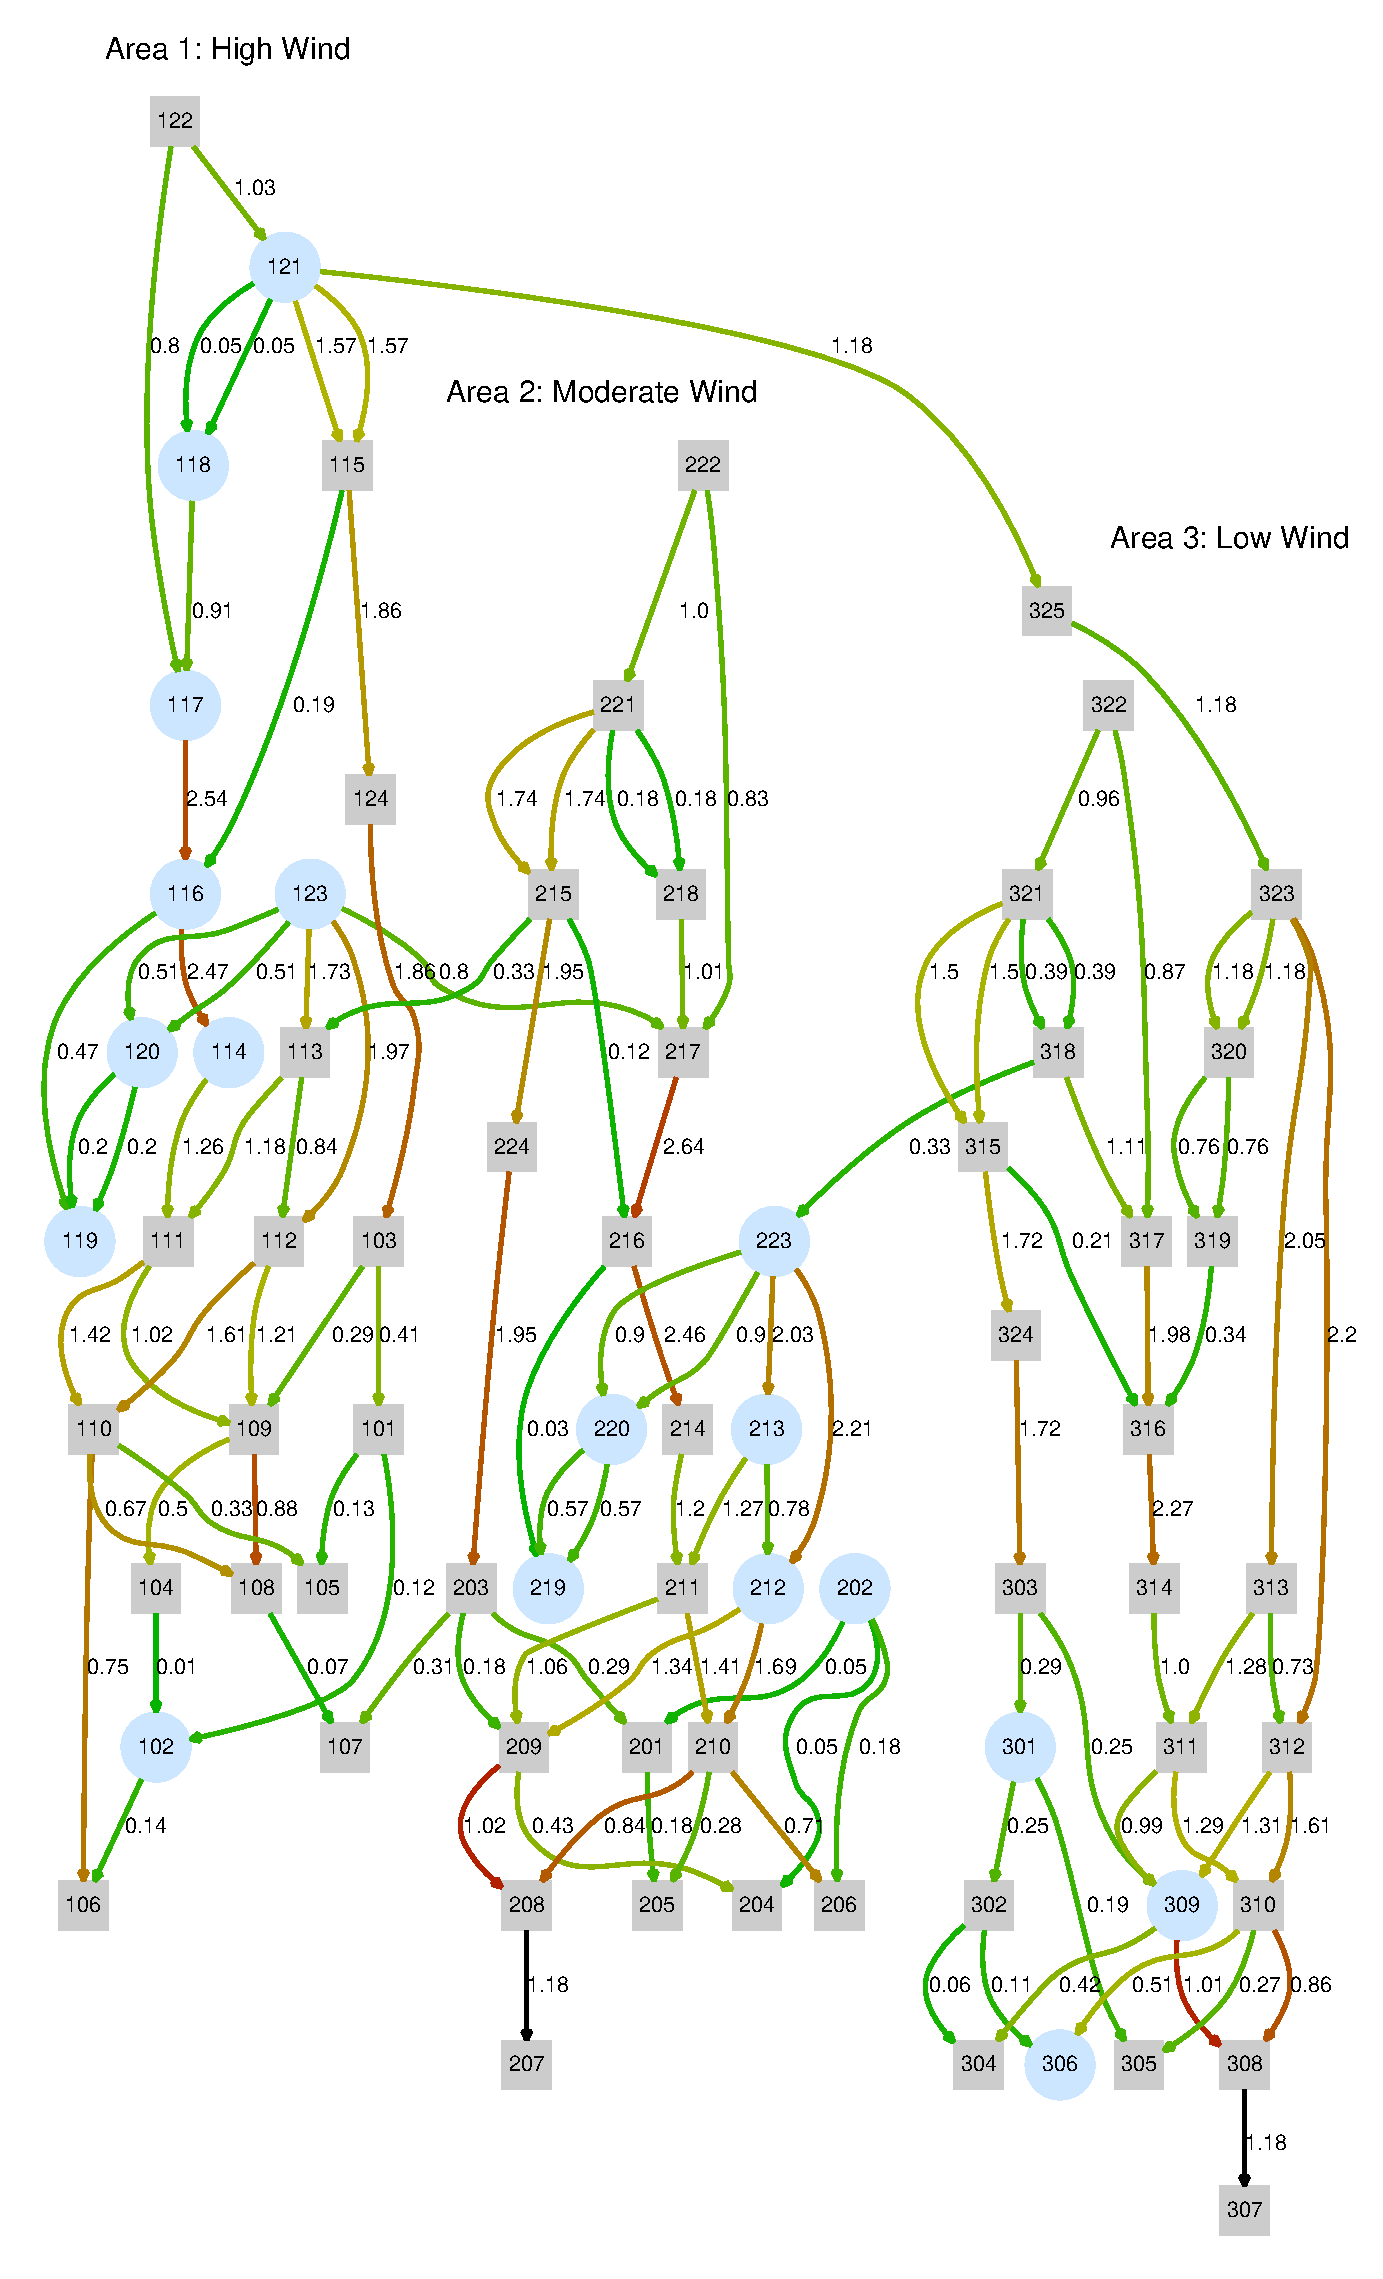
\includegraphics[width=1\linewidth]{images/line118}
\caption{Graph depiction of RTS-96 system state under instanton conditions at time step 2 of 3. The stressed line is between buses 121 and 325 (top center). wind-farms are indicated by blue, and lines are colored according to how close their flows are to static active power limits.}
\label{fig:line118}
\end{figure}


\section{Conclusions}

%The paper has extended instanton analysis to consider the temperature
%dynamics of overloaded lines. The resulting formulation is a
%quadratically constrained quadratic program (QCQP)\@. A
%computationally cheap algorithm has been developed for obtaining
%candidate solutions of this QCQP\@.  There is a great deal of
%flexibility in the temporal instanton model that has yet to be
%explored. In future work we plan to include transformers, consider the
%effects of ambient conditions in greater detail, and test the limits
%of the algorithm using larger networks with many time steps.

\section{Appendix: line temperature model}\label{sec:temp}

\subsection{The heat balance equation}

The change in temperature of any object may be expressed as a differential equation called the heat balance equation. This equation
relates temperature change to a sum of various sources of heating. The IEEE 738 standard \cite{ieee2013} provides the following heat balance equation for a transmission line:

\begin{align}\label{eq:heatbalance}
\frac{dT}{dt} &= \frac{1}{m\cdot C_p}\left[I^2\cdot R(T) - q_c - q_r + q_s \right]
\end{align}
where
\begin{itemize}
	\item $T$ is the conductor average temperature.
	\item $m\cdot C_p$ is the product of mass and heat capacity.
	\item $I^2\cdot R(T)$ represents heat rate due to resistive heating. In this paper the term is replaced by $f_{ij}^\text{loss}$, the DC approximate line loss expression derived in \cite{almassalkhi2014}.
	\item $q_c$ is the rate of heat loss due to convection. Any object at a higher temperature than surrounding air will gradually cool as the air carries heat away. This phenomenon is proportional to the temperature difference between the line and surrounding air:
		\begin{align}\label{eq:qc}
		q_c &= \eta_c\cdot(T - T_\text{amb})~,
		\end{align}
	where $T_\text{amb}$ is the ambient temperature (of surrounding air).
	\item $q_r$ is the rate of heat loss due to radiation. Thermal radiation is the process by which thermal energy is converted to electromagnetic energy in all objects with non-zero absolute temperature. It is modeled by a fourth-order expression:
	  \begin{align}\label{eq:qr}
	    q_r &= \eta_r\cdot\left[(T + 273)^4 - (T_\text{amb} + 273)^4\right]
	  \end{align}
	\item $q_s$ is the rate of heat gain due to solar heating. In this paper the solar heat rate is fixed to some conservative constant (representing full direct sun), but it is important to note that solar heat rate varies significantly with cloud cover, geometry, and even insulation type (reflective versus black).
\end{itemize}
%\begin{align}\label{eq:738heatbalance}
%\frac{dT_\text{avg}}{dt} &= \frac{1}{mC_p}\left( r_{ij}\frac{\theta_{ij}^2}{x_{ij}^2}\frac{S_b}{3L_{ij}} - q_c - q_r + q_s\right)
%\end{align}

\subsection{Linearization of radiation heat rate}

When \eqref{eq:heatbalance} is combined with an initial temperature $T_0$, the resulting initial value problem makes it possible to determine the temperature at any later time. Let's substitute the DC loss approximation, \eqref{eq:qc}, and \eqref{eq:qr} into \eqref{eq:heatbalance} and attempt to solve for temperature:

\begin{multline}
\frac{dT}{dt} = \frac{1}{mC_p}\big[ f_{ij}^\text{loss} - \eta_c\left( T(t) - T_\text{amb}\right) \\ - \eta_r\left((T(t) + 273)^4 - (T_\text{amb} + 273)^4\right) + q_s \big]
\end{multline}

Suppose that power flow, ambient temperature, and solar heat rate are constant during a temperature change calculation. There are just two variable terms on the right-hand side: one first-order, one fourth-order. The fourth-order term (which comes from $q_r$) makes this equation difficult to solve. Fortunately, $q_r$ is approximately linear over the temperature range we are interested in (from ambient to line limit). The figure below compares $q_r$ to a conservative\footnote{Because a transmission line is hotter than surrounding air, radiation tends to decrease line temperature. Thus, a conservative approach will underestimate the radiation heat rate, leading to slightly higher temperatures.} linearization $\tilde{q}_r$.

\begin{figure}[h]
\centering
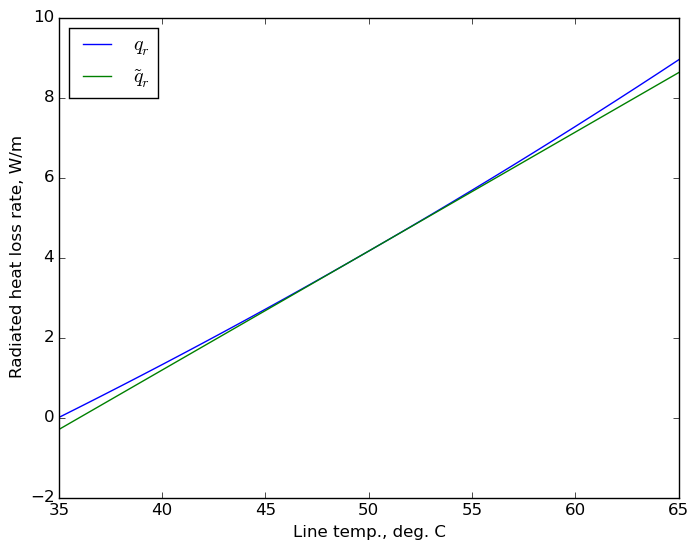
\includegraphics[width=0.9\linewidth]{../images/rad_approx}
\caption{Comparison of fourth-order radiation heat rate $q_r$ \eqref{eq:qr} with conservative linearization $\tilde{q}_r$ across a range of temperatures. Ambient temperature is 35$^\circ$C and the conductor thermal limit is 65$^\circ$C.}
\label{fig:rad_approx}
\end{figure}

The green trace is the linearization of $q_r$ about $T_\text{mid}$, the midpoint between the ambient and limit temperatures. Let's replace $q_r$ by this linear approximation $\tilde{q}_r$:

\begin{align}\label{eq:approx_qr}
\frac{dT}{dt} &= \frac{1}{mC_p}\left[ f_{ij}^\text{loss} - \eta_c\left( T(t) - T_\text{amb}\right) - \tilde{q}_r + q_s \right]
\end{align}

where

\begin{align}
\tilde{q}_r &= \eta_r  \left( (T_\text{mid} + 273)^4 - (T_\text{amb} + 273)^4\right) + 4\eta_r(T_\text{mid} + 273)^3\cdot(T(t) - T_\text{mid})
\end{align}


\subsection{Line temperature as IVP solution}
After simplification, \eqref{eq:approx_qr} becomes

\begin{align}\label{eq:diffeq}
\frac{dT}{dt} &= aT(t) + b
\end{align}

where constants $a$ and $b$ are defined as

\begin{subequations}
\begin{align}
a &= \frac{1}{mC_p} \left[ -\eta_c - 4\eta_r(T_\text{mid} + 273)^3 \right] \\
b &= \frac{1}{mC_p} \left[ f_{ij}^\text{loss} + \eta_cT_\text{amb} - \eta_r \left( (T_\text{mid} + 273)^4 - (T_\text{amb} + 273)^4 \right) + 4\eta_rT_\text{mid}(T_\text{mid} + 273)^3 + q_s \right]
\end{align}
\end{subequations}

The differential equation \eqref{eq:diffeq} has a straightforward solution:

\begin{align}\label{eq:tivp}
T(t) &= ke^{at} - \frac{b}{a}
\end{align}

where $k=T(0) + b/a$. Note that $b$ is influenced by power flow (via
$f_{ij}^\text{loss}$), but $a$ is not.    

\section{From temperature equation to optimization constraint}\label{from-ivp-to-optimization-constraint}

The important thing to note about the temperature equation \eqref{eq:tivp} is that it is influenced only by initial temperature and the angle difference during each time interval. There is therefore a recursive relationship between final temperature and initial temperature that involves only angle differences.

\subsection{Recursive relationship between final and initial temperatures}
Suppose there are three time intervals: $t_1$, $t_2$, and $t_3$. Then the line temperature at the end of the third interval is given by

\begin{align}
\nonumber T(t_3) &= k_3 e^{(t_3-t_2)a} - \frac{b_3}{a} \\
\nonumber &= \left[k_2 e^{(t_2-t_1)a} - \frac{b_2}{a} + \frac{b_3}{a}\right]e^{(t_3-t_2)a} - \frac{b_3}{a} \\
\nonumber &= \left[\left( T(t_1) + \frac{b_2}{a} \right)e^{(t_2-t_1)a} - \frac{b_2}{a} + \frac{b_3}{a}\right]e^{(t_3-t_2)a} - \frac{b_3}{a} \\
\label{eq:Texpand} &= \left\lbrace\left[\left(T(t_0) + \frac{b_1}{a}\right) e^{(t_1-t_0)a} - \frac{b_1}{a} + \frac{b_2}{a}\right]e^{(t_2-t_1)a} - \frac{b_2}{a} + \frac{b_3}{a}\right\rbrace e^{(t_3-t_2)a} - \frac{b_3}{a}
\end{align}
The recursive pattern is apparent. Because all time intervals are the same length, we have
\begin{align*}
e^{(t_3-t_2)a} &= e^{(t_2-t_1)a} = e^{(t_1-t_0)a}~,
\end{align*}
and we can distribute in \eqref{eq:Texpand} to obtain
\begin{align}
T(t_3) &= (e^{(t_1-t_0)a})^3\left(T(t_0) + \frac{b_1}{a}\right) + (e^{(t_1-t_0)a})^2\left(- \frac{b_1}{a} + \frac{b_2}{a}\right) + (e^{(t_1-t_0)a})\left(- \frac{b_2}{a} + \frac{b_3}{a}\right) - \frac{b_3}{a}
\end{align}
Because power flow data enters through $b_1$, $b_2$, and $b_3$, it makes sense to
group terms accordingly:

\begin{multline}
T(t_3) = ((e^{(t_1-t_0)a})^3T(t_0) + \left(\frac{(e^{(t_1-t_0)a})^3}{a} - \frac{(e^{(t_1-t_0)a})^2}{a}\right)b_1 + \\ + \left( \frac{(e^{(t_1-t_0)a})^2}{a} - \frac{(e^{(t_1-t_0)a})^1}{a}\right)b_2 + \left(\frac{e^{(t_1-t_0)a}}{a} - \frac{1}{a}\right) b_3
\end{multline}
The pattern in the above expression makes it easy to extend $T(t_3)$ to cover the general case $T(t_n)$:

\begin{align}\label{eq:recursive}
T(t_n) &= (e^{(t_1 - t_0)a})^n T(t_0) + \frac{1}{a} \sum_{i=1}^n \left( (e^{(t_1-t_0)a})^i - (e^{(t_1-t_0)a})^{i-1} \right)b_{n-i+1}
\end{align}

Ultimately \eqref{eq:recursive} will be used to constrain a line's final temperature to some limiting value. The remainder of this section will relate \eqref{eq:recursive} back to power flow angles so it can be ``plugged in'' to the optimization framework.

\subsection{Relating temperature to angle differences}

Recall that $b_n$ depends on the angle difference at time $t_n$:

\begin{align}
\nonumber b_n &= \frac{1}{mC_p} \left[ \frac{r_{ij}}{x_{ij}^2}\cdot \frac{S_b}{3L_{ij}} \theta_{ij}(t_n)^2 + \eta_cT_\text{amb} - \eta_r\left((T_\text{mid} + 273)^4 - (T_\text{amb} + 273)^4\right) + 4\eta_rT_\text{mid}(T_\text{mid} + 273)^3 + q_s \right] \\
\label{eq:bexpand} b_n &= c\theta_{ij}(t_n)^2 + d
\end{align}
where constants $c$ and $d$ are defined as:
\begin{align*}
c &= \frac{r_{ij}S_b}{3 mC_p x_{ij}^2L_{ij}} \\
 d &= \frac{1}{mC_p}\left[ \eta_cT_\text{amb} - \eta_r\left((T_\text{mid} + 273)^4 - (T_\text{amb} + 273)^4\right) + 4\eta_rT_\text{mid}(T_\text{mid} + 273)^3 + q_s \right]
\end{align*}
Substitute \eqref{eq:bexpand} into \eqref{eq:recursive}:
\begin{align*}
T(t_n) &= (e^{(t_1 - t_0)a})^n T(t_0) + \frac{1}{a} \sum_{i=1}^n \left( (e^{(t_1-t_0)a})^i - (e^{(t_1-t_0)a})^{i-1} \right)(c\theta_{ij}(t_{n-i+1})^2 + d)
\end{align*}
Expand the sum term:
\begin{multline}\label{eq:sumexpand}
\frac{1}{a} \sum_{i=1}^n \left( (e^{(t_1-t_0)a})^i - (e^{(t_1-t_0)a})^{i-1} \right)(c\theta_{ij}(t_{n-i+1})^2 + d) = \frac{c}{a}\left[ \sum_{i=1}^n \left( (e^{(t_1-t_0)a})^i - (e^{(t_1-t_0)a})^{i-1} \right)\theta_{ij}(t_{n-i+1})^2\right] + \\  \qquad + \frac{d}{a}\left[ \sum_{i=1}^n \left( (e^{(t_1-t_0)a})^i - (e^{(t_1-t_0)a})^{i-1} \right)\right] 
\end{multline}
Substitute \eqref{eq:sumexpand} into the line temperature equation, introducing the constant $f$ to keep things a bit neater:
\begin{align}\label{eq:almostthere}
T(t_n) &= f + \frac{c}{a}\left[ \sum_{i=1}^n \left( (e^{(t_1-t_0)a})^i - (e^{(t_1-t_0)a})^{i-1} \right)\theta_{ij}(t_{n-i+1})^2\right]
\end{align}
where
\begin{align}
f &= (e^{(t_1 - t_0)a})^n T(t_0) + \frac{d}{a}\left[ \sum_{i=1}^n \left( (e^{(t_1-t_0)a})^i - (e^{(t_1-t_0)a})^{i-1} \right)\right]
\end{align}
Rearrange \eqref{eq:almostthere} to isolate angle differences:
\begin{align}
\sum_{i=1}^n \left( (e^{(t_1-t_0)a})^i - (e^{(t_1-t_0)a})^{i-1} \right)\theta_{ij}(t_{n-i+1})^2 &= \frac{a}{c}(T(t_n) - f)
\end{align}
Now define
\begin{equation}\label{eq:thetahat}
\hat{\theta}_{ij}(t_{k})=  \theta_{ij}(t_k)\sqrt{ (e^{(t_1-t_0)a})^{n-k+1} - (e^{(t_1-t_0)a})^{n-k} }
\end{equation}
to obtain
\begin{align}\label{eq:finaltemp}
\sum_{k=1}^n \hat{\theta}_{ij}(t_{k})^2 &= \frac{a}{c}\left(T(t_n) - f\right)
\end{align}
The expression \eqref{eq:finaltemp} may be used to constrain line temperature to be equal to some limiting value by the end of the last time interval.

This derivation has been somewhat messy. The line temperature constraint is summarized in the next section for convenience.

\subsection{Summary of line temperature constraint}\label{summary-of-line-temperature-constraint}

Suppose our time horizon consists of $n$ intervals, each on the order of
ten minutes long. Power flow data is updated after each interval, but
all other parameters remain constant. Choose a single transmission
line in the network, and suppose it lies between nodes $i$ and $j$. This line has a
thermal limit of $T_\text{lim}$ ($^\circ$C). We can constrain the
line's temperature to be equal to this limiting value by enforcing the
second-order constraint:

\begin{align}\label{eq:tempconstraint}
\sum_{k=1}^n \hat{\theta}_{ij}(t_k)^2 &= \frac{a}{c}\left(T_\text{lim} - f\right)
\end{align}

where

\begin{itemize}
\itemsep1pt\parskip0pt\parsep0pt
\item
  $\hat{\theta}_{ij}(t_{k})=  \theta_{ij}(t_k)\sqrt{ (e^{(t_1-t_0)a})^{n-k+1} - (e^{(t_1-t_0)a})^{n-k} } $

  \begin{itemize}
  \itemsep1pt\parskip0pt\parsep0pt
  \item
    $\theta_{ij}(t_k)$ is the angle difference across line $ij$ at time
    interval $t_k$.
  \item
    $(t_1-t_0)$ is the length of each time interval (in seconds)
  \end{itemize}
\item
  $ a =
  \frac{1}{mC_p}\left[ -\eta_c - 4\eta_r(T_\text{mid} + 273)^3 \right]$
  is constant with units of $s^{-1}$

  \begin{itemize}
  \itemsep1pt\parskip0pt\parsep0pt
  \item
    $mC_p$ is the heat capacity, with units of J/m-$^\circ$C
  \item
    $\eta_c$ is the conductive heat loss rate coefficient, with units of
    W/m-$^\circ$C
  \item
    $\eta_r$ is the conductive heat loss rate coefficient, with units of
    W/m-$^\circ$C$^4$
  \item
    $T_\text{mid}$ is the average of ambient temperature $T_\text{amb}$
    and limit temperature $T_\text{lim}$, in Celsius
  \end{itemize}
\item
  $c = \frac{r_{ij}S_b}{3 mC_p x_{ij}^2L_{ij}}$ is a constant with units
  of W/m

  \begin{itemize}
  \itemsep1pt\parskip0pt\parsep0pt
  \item
    $r_{ij}$ is resistance of line $ij$ in per unit
  \item
    $x_{ij}$ is reactance of line $ij$ in per unit
  \item
    $S_b$ is the system base (e.g.~100 MVA)
  \item
    $L_{ij}$ is the length of one phase of line $ij$, in m
  \end{itemize}
\item
  $f = (e^{(t_1 - t_0)a})^n T(t_0) + \frac{d}{a}\left[ \sum_{i=1}^n \left( (e^{(t_1-t_0)a})^i - (e^{(t_1-t_0)a})^{i-1} \right)\right]$
  is a constant with units of degrees Celsius

  \begin{itemize}
  \itemsep1pt\parskip0pt\parsep0pt
  \item
    $T(t_0)$ is the line's initial temperature (steady state temperature
    under base case power flow condition)
  \item
    $d = \frac{1}{mC_p}\left[ \eta_cT_\text{amb} - \eta_r\left((T_\text{mid} + 273)^4 - (T_\text{amb} + 273)^4\right) + 4\eta_rT_\text{mid}(T_\text{mid} + 273)^3 + q_s \right]$
    is a constant with units of W/m

    \begin{itemize}
    \itemsep1pt\parskip0pt\parsep0pt
    \item
      $q_s$ is the solar heat gain rate in W/m
    \end{itemize}
  \end{itemize}
\end{itemize}



\section{Numerical comparison to IEEE 738 standard model}\label{numerical-comparison-of-temperature-models}

To validate the approximate line temperature model derived here, I compared it to the IEEE 738 standard model using RTS-96 and Waxwing conductor parameters.

\subsection{Summary of IEEE 738 temperature calculation}\label{summary-of-ieee-738-temperature-calculation}

IEEE recommends numerically integrating \eqref{eq:heatbalance} to compute temperature changes. The temporal instanton framework uses approximate DC losses in place of $I^2R(T_\text{avg})$, so we will be integrating the following heat balance equation:

\begin{align}\label{eq:738heatbalance}
\frac{dT_\text{avg}}{dt} &= \frac{1}{mC_p}\left( r_{ij}\frac{\theta_{ij}^2}{x_{ij}^2}\frac{S_b}{3L_{ij}} - q_c - q_r + q_s\right)
\end{align}

Heat rates $q_c$ and $q_r$ are calculated according to \eqref{eq:qc} and \eqref{eq:qr}, respectively (copied here for convenience):
\begin{align*}
q_c &= \eta_c\cdot(T - T_\text{amb}) \\
q_r &= \eta_r\cdot((T + 273)^4 - (T_\text{amb} + 273)^4)
\end{align*}
All other parameters are constant during temperature calculation. The important thing to keep in mind about IEEE 738 temperature calculation is that it requires numerical integration; there is no analytic temperature solution for \eqref{eq:738heatbalance}. This means one must select an integration time step $\Delta t$. For each step, one computes the change in temperature by multiplying $\Delta t$ by the value of \eqref{eq:738heatbalance} computed at that step. IEEE recommends a step size smaller than 10\% of the conductor thermal time constant\footnote{A typical transmission line thermal time constant is ten minutes, which means IEEE recommends an integration step size of one minute}. A smaller integration step size yields more accurate results.

\subsection{Comparison}\label{comparison}

I used RTS-96 network data and Waxwing conductor parameters to compare IEEE 738 standard temperature calculation to the model derived in Section \ref{transmission-line-heating}. Figure \ref{fig:temp_model_comparison2} shows line temperatures calculated across three ten-minute time intervals, where each interval has a different angle difference (power flow). The angle differences are
\begin{center}
\begin{tabular}{c|c}
	Interval & Angle difference (rad) \\ \hline
	   1     &          0.09          \\ 
	   2     &          0.04          \\ 
	   3     &          0.15          \\ 
\end{tabular} 
\end{center}

\begin{figure}[h]
\centering
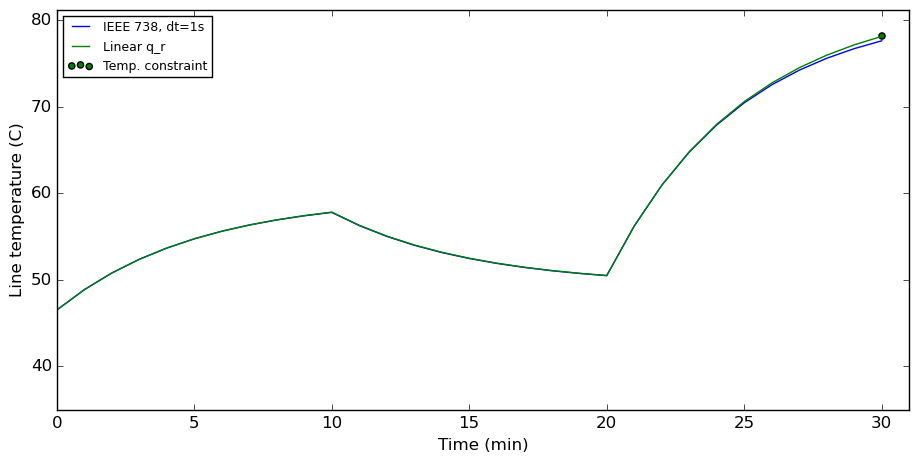
\includegraphics[width=1\linewidth]{../images/temp_model_comparison2}
\caption{Comparison of IEEE 738 and approximate temperature calculation methods}
\label{fig:temp_model_comparison2}
\end{figure}

The blue trace in Figure \ref{fig:temp_model_comparison2} results from numerical integration of \eqref{eq:738heatbalance} with a 1s step size. The green trace comes from the approximate model derived in Section \ref{transmission-line-heating}. The green dot is the final temperature computed by \eqref{eq:almostthere}.

Notes:

\begin{itemize}
\item
  Because the approximate line temperature model is analytic (Equation \eqref{eq:tivp} is continuous) while the 738 model requires numerical integration, I chose
  a very small integration step size of one second to facilitate comparison.
\item
  Because the approximate model underestimates the radiative heat loss
  rate (see Figure \ref{fig:rad_approx}), the green trace should lie slightly above the blue one. This
  makes the approximate model conservative, which is desirable in the
  temporal instanton setting. Figure \ref{fig:temp_model_comparison2} illustrates this conservative behavior: the green trace lies on or above the blue trace throughout the time horizon.
  \item The green dot, computed by \eqref{eq:almostthere}, lies on top of the green curve. This validates the temperature constraint formulation \eqref{eq:tempconstraint}.
\end{itemize}

\subsection{Line temperature dynamics}\label{sec:temp-dynamics}

%Section \ref{sec:line-losses} describes an approximate line loss formulation that forms the basis of a dynamical model developed in Section \ref{sec:temp-dynamics}. Finally, Section \ref{sec:instanton-formulation} incorporates line temperature dynamics into a complete mathematical model.

%The equations governing AC power flow are nonlinear. If we use these equations to balance the power flows in our optimization, the resulting feasible region will be nonconvex. Previous instanton work has addressed this issue by replacing the AC power flow equations with DC equations (the DC power flow equations assume that the network is lossless, with all voltage magnitudes equal to 1 per unit). This substitution renders the feasible region of instanton optimization (in the absence of nonlinear constraints) convex. 

%There are two primary difficulties associated with time-coupled instanton analysis. First, every active and reactive power flow is related to all variables involved in the flow:  the voltage magnitudes at both nodes and the angle difference between them. If we allow this tight coupling into our optimization framework, there will be no guarantee of a unique solution, or indeed of any solution at all. The second difficulty arises from the equation for power loss. Power loss on a line is proportional to the square of the current through it. This nonlinear relationship leads to nonconvexity in the optimization problem's feasible region. In this paper we address the first concern by using the DC power flow, and we sidestep the second difficulty by using a piecewise-continuous convex relaxation of the power loss equation.


\newcommand{\splitcell}[2][c]{%
\begin{tabular}[#1]{@{}c@{}}#2\end{tabular}}
\begin{table}
\begin{center}
\caption{Line heating parameters}
\label{tab:heatparams}
\begin{tabular}{|c|c|c|}
	\hline
	         Parameter           &   Units    &               Description                \\ \hline
	           $T_s$             &    $s$     &               Sample time                \\ \hline
	           $mC_p$            & $J/(m\cdot C)$ & \splitcell{Per-unit-length heat capacity\\of the conductor}         \\ \hline
	          $\eta_c$           & $W/(m\cdot C)$ &     \splitcell{Conductive heat loss \\ rate coefficient}         \\ \hline
	          $\eta_r$           & $W/(m\cdot C)$ &      \splitcell{Radiative heat loss\\rate coefficient}         \\ \hline
	       $T^\text{lim}$        &    $C$     &      \splitcell{Line temperature at\\steady-state current limit.}   \\ \hline
	       $\Delta q_{s,ij}$ & $W/m$ & \splitcell{Solar heat input\\ into conductor} \\ \hline
	       $\Delta T_\text{amb}$ & C & \splitcell{Change in \\ambient temperature} \\ \hline
\end{tabular} 
\end{center}
\end{table}

\subsection{Instanton formulation}\label{sec:instanton-formulation}

The preceding discussion developed an approximate line loss expression
to relate line temperature to angle variables according to
\eqref{TD:vectors}. Here we describe the remaining parts of the
temporal instanton model.

The following equations describe an optimization problem that
minimizes deviation from the wind forecast while heating a certain
line to a specified (limiting) temperature:
\begin{subequations}\label{I:all}
\begin{align}
\label{I:obj}\underset{dev}{\min} \quad & \sum_{t=1}^{T} dev_t^\top Q_{dev} dev_t \\
\nonumber \text{subject to:} & \\
\label{I:flow} \sum_j Y_{ij} \theta_{ij,t} & = G_{i,t} + R_{i,t} +
dev_{i,t} - D_{i,t} \\[-8pt]
\nonumber &\qquad\qquad\qquad\quad \forall i \in 1... N,~t\in 1... T \\%[6pt]
\label{I:conv} G_t &= G_{0,t} + k\alpha_t \quad\: \forall t\in 1\ldots T \\
\label{I:slack} \theta_{ref,t} & = 0 \qquad\qquad\quad\; \forall t\in 1\ldots T \\
\label{I:lim} \Delta T_{ij}[T] &= \Delta T_{ij}^\text{lim}\qquad\quad\: \text{for some }(i,j)\in \mathcal{G}
\end{align}
\end{subequations}
where:
\begin{itemize}
\itemsep1pt\parskip0pt\parsep0pt
\item $dev_{i,t}$ is the difference between actual output and forecast output at wind-farm $i$ and time $t$. Thus, $dev_t$ is the vector of wind forecast deviations at time $t$.
\item $Q_{dev}$ may be set to the identity matrix or used to encode correlation between wind sites.
\item $R_{i,t}$ is renewable generation forecast at bus $i$ and time $t$.
\item $Y_{ij}$ is the $(i,j)$-th element of the admittance matrix, which assumes zero resistance.
\item $\theta_{ij,t}$ is the difference between voltage angles $\theta_i$ and $\theta_j$ at time $t$.
\item $G_{i,t}$ is conventional active power generation at node $i$ and time $t$, and $G_t$ is a vector including all nodes.
\item $D_{i,t}$ is active power demand at bus $i$ and time $t$.
\item $N$ is the number of buses (nodes).
\item $G_{0,t}$ is scheduled conventional active power generation (without droop response).
\item $k$ is the vector of participation factors for conventional generators, with $\sum_i k_i = 1$. (The case where $k_i=1$ corresponds to generator $i$ taking all slack.)
\item $\alpha_t$ is the power mismatch at time $t$.
\item $\Delta T_{ij}^{lim}$ is the change in temperature that will push line $(i,j)$ to its thermal limit.
\item $\theta_\text{ref}$ is the voltage angle of the reference bus.
\item $\mathcal{G}$ is the set of edges (lines).
\end{itemize}

Equation \eqref{I:obj} expresses the desire to find wind patterns that
remain close to the wind forecast. The first constraint equation
\eqref{I:flow} enforces DC power balance. The next constraint
\eqref{I:conv} models conventional active power generation as a sum of
scheduled generation and droop response (where generators share the
task of compensating for mismatch between total generation and
load). The system angle reference is established by
\eqref{I:slack}. Last is \eqref{I:lim}, which constrains the
temperature of a particular line to be equal to its limit at the final
time $T$. Using \eqref{TD:vectors} we can express
\eqref{I:lim} as
\begin{align}\label{temp}
\Delta T_{ij}^{\text{lim}} - \delta_{ij} \boldsymbol{\Delta d}_{ij}^\top \boldsymbol{\tau}_{ij}\mathbf{1}   &= \frac{\rho_{ij}r_{ij}}{x_{ij}^2} \boldsymbol{\theta}_{ij}^\top \boldsymbol{\tau}_{ij} \boldsymbol{\theta}_{ij}.
\end{align}
Thus, \eqref{I:all} has a quadratic objective function, a set of linear constraints, and a single quadratic constraint. By solving \eqref{I:all} for each line in the network, we obtain a set of instanton candidate wind patterns, each of which will heat a particular line to its thermal limit. Of these candidates, the one that deviates least from the wind forecast (across all time steps) is the instanton wind pattern.

The form of \eqref{I:all} suggests a QCQP optimization
formulation. The next section establishes this QCQP.

\section{Conversion to optimization problem}\label{sec:optimization}

Previous instanton work relied on convex optimization to quickly find instanton wind patterns. Heat-constrained temporal instanton analysis is more complicated:  it cannot be formulated as anything simpler than a quadratically-constrained quadratic program (QCQP). QCQPs are NP-hard in general; reasonable solutions may exist, but unless the quadratic constraint matrices are positive-definite there is no solution guarantee (see \cite{mehanna2014}). Because system operators require robustness, ``no solution found'' is an unacceptable output. With this criterion in mind, we proceed to develop an optimization model whose structure permits us to find solutions despite nonconvexity.

With all deviation, angle, and mismatch variables stacked into a single vector, \eqref{I:all} takes the form:
\begin{subequations}\label{opt}
\begin{align}
\label{opt:obj} \min\quad z^\top &Q_{obj} z \\
\label{opt:lin}  s.t.\quad Az &= b  \\
\label{opt:quad}  z^\top Q_{\theta}z &= c.
\end{align}
\end{subequations}
The objective \eqref{opt:obj} is equivalent to \eqref{I:obj}, the
linear equality constraints \eqref{opt:lin} represent
\eqref{I:flow}-\eqref{I:slack}, and the quadratic equality constraint
\eqref{opt:quad} is equivalent to \eqref{I:lim}. The vector $z$
consists of $(N+N_R+2)T$ variables, where $N$ is the number of nodes,
$N_R$ is the number of nodes with wind-farms, and $T$ is the number of
time steps. Note that $N_RT$ of the variables represent deviations
from forecast at each wind-farm and time step. There are also $NT$
angle variables (of which $T$ are fixed to zero according to
\eqref{I:slack}) and $T$ mismatch variables $\alpha_t$ (one per time
step). The last $T$ variables are auxiliary angle difference variables
used to convert \eqref{I:lim} into a norm constraint; they are defined
later in \eqref{thetahat}.

Variables may be stacked in any order. One convenient ordering is $T$
groups of $(N+N_R+1)$ variables, with the $T$ auxiliary angle
difference variables at the end. At a particular time step $t$, the
group of $(N+N_R+1)$ variables is $[dev_t^\top ~~ \theta_t^\top ~~
  \alpha_t ]^\top$, with $dev_t$ representing deviations from forecast
at the $N_R$ wind nodes, $\theta_t$ is the column of $N$ angle
variables at time $t$, and $\alpha_t$ is the mismatch between
generation and demand at time $t$.

The remainder of this section describes the components of
\eqref{opt}. The objective matrix $Q_{obj}$ is described in
Section~\ref{sec:Qobj}, linear constraint parameters $A$ and $b$ are
considered in Section~\ref{sec:Ax=b}, and the constraint matrix
$Q_{\theta}$ is addressed in Section~\ref{sec:Qtheta}.

% The paper will close with a discussion of how other
%components, such as voltage regulators, may affect the formulation.

%\section*{Acknowledgment}

%\section*{References}

% can use a bibliography generated by  as a .bbl file
% BibTeX documentation can be easily obtained at:
% http://www.ctan.org/tex-archive/biblio/bibtex/contrib/doc/
% The IEEEtran BibTeX style support page is at:
% http://www.michaelshell.org/tex/ieeetran/bibtex/
\bibliographystyle{IEEEtran}
% argument is your BibTeX string definitions and bibliography database(s)
%\bibliography{IEEEabrv,../bib/paper}
\bibliography{bib}

\end{document}


